\documentclass[border=12pt]{standalone}
\def\pgfsysdriver{pgfsys-dvisvgm.def}
\usepackage[dvisvgm]{xcolor}
\usepackage{xeCJK}
\setCJKmainfont{HaranoAjiGothic-Regular.otf}[BoldFont=HaranoAjiGothic-Bold.otf]
\setCJKsansfont{HaranoAjiGothic-Regular.otf}[BoldFont=HaranoAjiGothic-Bold.otf]
\usepackage{amsmath,amssymb,tikz,lmodern}
\usetikzlibrary{arrows.meta,positioning,calc,fit,backgrounds}
\renewcommand{\familydefault}{\sfdefault}
\definecolor{ink}{HTML}{25322F}
\definecolor{green}{HTML}{246657}
\definecolor{tint}{HTML}{EEF4F0}
\definecolor{soft}{HTML}{C6D2CC}
\definecolor{muted}{HTML}{52615B}
\newif\ifJapanese
\newcommand{\Tx}[2]{\ifJapanese #1\else #2\fi}
\newcommand{\Eff}{\overline{\operatorname{Eff}}}
\newcommand{\heading}[3]{{\color{green}\bfseries #1\quad\Tx{#2}{#3}}\\[5pt]}
% A white rectangle makes the complete citation label clickable, including spaces.
\newcommand{\refurl}[2]{\special{dvisvgm:raw <a xlink:href="#1" target="_blank" rel="noopener noreferrer">}{\setlength{\fboxsep}{0pt}\colorbox{white}{\color{green}\underline{\strut #2}}}\special{dvisvgm:raw </a>}}
\newcommand{\refedge}[3]{\refurl{\csname source#1\endcsname\string##page=#2}{#3}}
\newcommand{\SF}[2]{\refedge{sf}{#1}{#2}}
% GitHub's file preview does not support PDF page fragments.
\newcommand{\LA}[2]{\refurl{\sourcela}{#2}}
\newcommand{\Sch}[2]{\refedge{sch}{#1}{#2}}
\newcommand{\PS}[2]{\refedge{ps}{#1}{#2}}
\tikzset{
 card/.style={draw=soft,fill=white,rounded corners=2pt,align=left,text=ink,font=\fontsize{10.5}{14}\selectfont,inner xsep=12pt,inner ysep=10pt,text width=14.4cm},
 half/.style={card,text width=6.45cm,minimum height=2.05cm},
 result/.style={card,draw=green,fill=tint,line width=.9pt},
 reason/.style={align=left,text=muted,font=\fontsize{9}{12}\selectfont,inner sep=0pt,text width=12.7cm},
 branchreason/.style={reason,text width=5.95cm},
 edge/.style={-{Stealth[length=2.4mm]},draw=green,line width=1pt},
 wire/.style={draw=green,line width=1pt},
}
% Keep the arrow in a dedicated left gutter; explanations never cover it.
\newcommand{\flow}[3]{
 \coordinate (#2-from) at ($(#1.south)+(-6.9,0)$);
 \coordinate (#2-to) at ($(#2.north)+(-6.9,0)$);
 \draw[edge] (#2-from)--(#2-to);
 \node[reason,anchor=west] (#2-reason) at ($(#2-from)!.5!(#2-to)+(.55,0)$) {#3};
}
\newcommand{\Cite}[2]{\refurl{\csname source#1\endcsname}{#2}}

\Japanesefalse
\newcommand{\sourcefn}{https://github.com/openai/math/blob/adc7f1241b42e322a6451854ab7e4b4c146bf78a/preprints/Fourfold-nonvanishing-by-minimal-metrics-and-moving-jets-September-27-2026/paper.pdf}
\newcommand{\sourcemm}{https://github.com/openai/math/blob/adc7f1241b42e322a6451854ab7e4b4c146bf78a/preprints/Minimal-metrics-and-interior-injectivity-for-nef-adjoints-September-27-2026/paper.pdf}
\newcommand{\sourcela}{https://github.com/openai/math/blob/adc7f1241b42e322a6451854ab7e4b4c146bf78a/preprints/Log-abundance-in-characteristic-zero-September-24-2026/paper.pdf}
\newcommand{\sourcelift}{https://github.com/openai/math/blob/adc7f1241b42e322a6451854ab7e4b4c146bf78a/preprints/Lifting-sections-from-the-reduced-support-of-an-adjoint-September-27-2026/paper.pdf}
\newcommand{\sourcect}{https://arxiv.org/pdf/2011.02236v2}
\newcommand{\sourcefuj}{https://www.math.kyoto-u.ac.jp/~fujino/Abundance.pdf}
\newcommand{\sourcegm}{https://arxiv.org/pdf/1406.6132v2}
\newcommand{\sourcehash}{https://arxiv.org/pdf/1609.00121v4}
\begin{document}
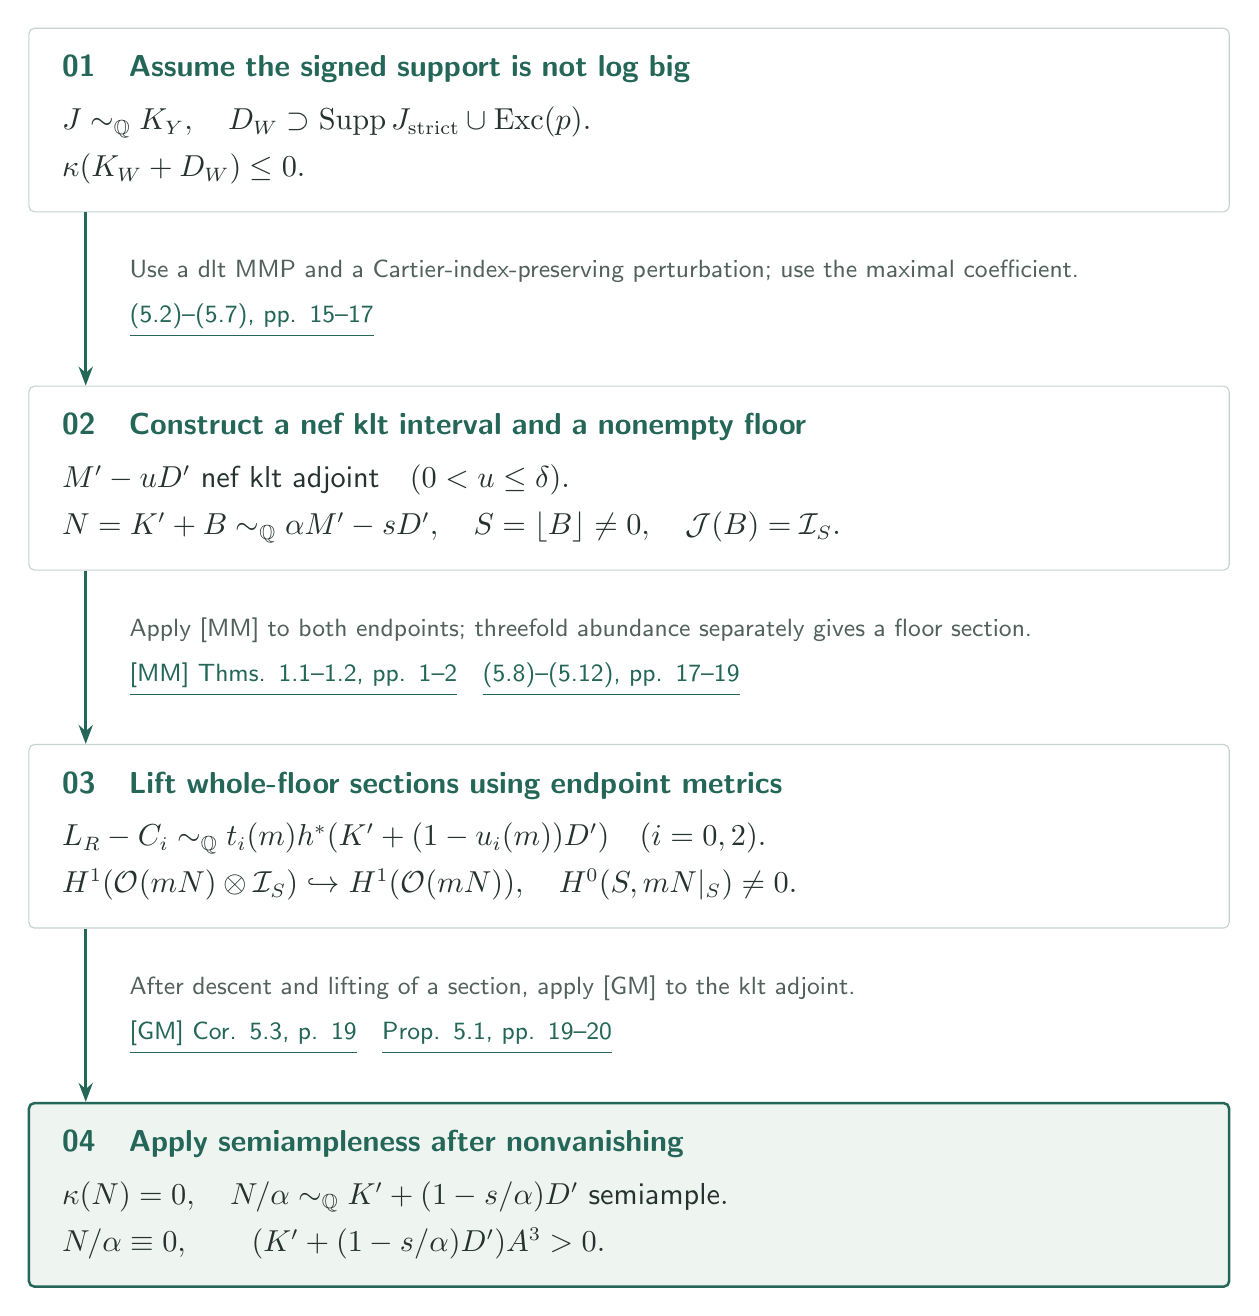
\begin{tikzpicture}
\node[card] (n0) {\heading{01}{符号付き代表の台がbigでないと仮定する}{Assume the signed support is not log big}\Tx{$J\sim_{\mathbb Q}K_Y,\quad D_W\supset\operatorname{Supp}J_{\rm strict}\cup\operatorname{Exc}(p).$\\[3pt]$\kappa(K_W+D_W)\le0.$}{$J\sim_{\mathbb Q}K_Y,\quad D_W\supset\operatorname{Supp}J_{\rm strict}\cup\operatorname{Exc}(p).$\\[3pt]$\kappa(K_W+D_W)\le0.$}};
\node[card,below=2.2cm of n0] (n1) {\heading{02}{nef klt区間と非空のfloorを構成する}{Construct a nef klt interval and a nonempty floor}\Tx{$M^{\prime}-uD^{\prime}\text{ nef klt adjoint}\quad(0<u\le\delta).$\\[3pt]$N=K^{\prime}+B\sim_{\mathbb Q}\alpha M^{\prime}-sD^{\prime},\quad S=\lfloor B\rfloor\ne0,\quad\mathcal J(B)=\mathcal I_S.$}{$M^{\prime}-uD^{\prime}\text{ nef klt adjoint}\quad(0<u\le\delta).$\\[3pt]$N=K^{\prime}+B\sim_{\mathbb Q}\alpha M^{\prime}-sD^{\prime},\quad S=\lfloor B\rfloor\ne0,\quad\mathcal J(B)=\mathcal I_S.$}};
\flow{n0}{n1}{\Tx{dlt MMPとCartier指数を保つcrepant摂動。最大正係数でfloorを作る。}{Use a dlt MMP and a Cartier-index-preserving perturbation; use the maximal coefficient.}\\[4pt]\Cite{fn}{(5.2)--(5.7), pp. 15--17}}
\node[card,below=2.2cm of n1] (n2) {\heading{03}{端点計量で全floorからの切断を持ち上げる}{Lift whole-floor sections using endpoint metrics}\Tx{$L_R-C_i\sim_{\mathbb Q}t_i(m)h^*(K^{\prime}+(1-u_i(m))D^{\prime})\quad(i=0,2).$\\[3pt]$H^1(\mathcal O(mN)\otimes\mathcal I_S)\hookrightarrow H^1(\mathcal O(mN)),\quad H^0(S,mN|_S)\ne0.$}{$L_R-C_i\sim_{\mathbb Q}t_i(m)h^*(K^{\prime}+(1-u_i(m))D^{\prime})\quad(i=0,2).$\\[3pt]$H^1(\mathcal O(mN)\otimes\mathcal I_S)\hookrightarrow H^1(\mathcal O(mN)),\quad H^0(S,mN|_S)\ne0.$}};
\flow{n1}{n2}{\Tx{二端点に [MM] を適用。全floorの非零切断には別途三次元abundanceを使う。}{Apply [MM] to both endpoints; threefold abundance separately gives a floor section.}\\[4pt]\Cite{mm}{[MM] Thms. 1.1--1.2, pp. 1--2}\quad \Cite{fn}{(5.8)--(5.12), pp. 17--19}}
\node[result,below=2.2cm of n2] (n3) {\heading{04}{非消滅後の半豊富性で矛盾を得る}{Apply semiampleness after nonvanishing}\Tx{$\kappa(N)=0,\quad N/\alpha\sim_{\mathbb Q}K^{\prime}+(1-s/\alpha)D^{\prime}\text{ semiample}.$\\[3pt]$N/\alpha\equiv0,\qquad (K^{\prime}+(1-s/\alpha)D^{\prime})A^3>0.$}{$\kappa(N)=0,\quad N/\alpha\sim_{\mathbb Q}K^{\prime}+(1-s/\alpha)D^{\prime}\text{ semiample}.$\\[3pt]$N/\alpha\equiv0,\qquad (K^{\prime}+(1-s/\alpha)D^{\prime})A^3>0.$}};
\flow{n2}{n3}{\Tx{切断を降下・持ち上げた後、klt随伴へ [GM] を適用する。}{After descent and lifting of a section, apply [GM] to the klt adjoint.}\\[4pt]\Cite{gm}{[GM] Cor. 5.3, p. 19}\quad \Cite{fn}{Prop. 5.1, pp. 19--20}}
\end{tikzpicture}
\end{document}
